% TGC resistive readout — schematic of the *implemented* signal chain
% (as coded in src/tgc_sim.cc for config/default_tgc.json).
% Compile: pdflatex readout_scheme.tex
\documentclass[11pt]{article}
\usepackage[margin=1.8cm]{geometry}
\usepackage{tikz}
\usepackage{amsmath}
\usepackage{xcolor}
\usepackage{graphicx}
\usetikzlibrary{positioning,arrows.meta,calc,fit,backgrounds}

% red circled criticality marker, e.g. \crit{1}
\newcommand{\crit}[1]{\tikz[baseline=(c.base)]{%
  \node[circle,draw=red!75!black,fill=red!12,line width=0.4pt,inner sep=1.2pt] (c)
  {\scriptsize\bfseries #1};}}
\tikzset{
  layer/.style={draw=black,thick},
  blk/.style={draw=black,thick,rounded corners=2pt,align=center,
              minimum height=10mm,minimum width=20mm,font=\small,fill=blue!4},
  hp/.style ={blk,fill=orange!12},
  lp/.style ={blk,fill=cyan!10},
  sig/.style={-{Latex[length=2mm]},thick},
  critmark/.style={circle,draw=red!75!black,fill=red!12,line width=0.5pt,
                   inner sep=1.3pt,font=\scriptsize\bfseries},
}
% discrete-component pics for the electronics schematic (plain TikZ; no circuitikz)
\tikzset{
  caph/.pic={\draw[thick](-0.45,0)--(-0.08,0) (-0.08,-0.22)--(-0.08,0.22)
                         (0.08,-0.22)--(0.08,0.22) (0.08,0)--(0.45,0);},
  capv/.pic={\draw[thick](0,0.45)--(0,0.08) (-0.22,0.08)--(0.22,0.08)
                         (-0.22,-0.08)--(0.22,-0.08) (0,-0.08)--(0,-0.45);},
  resh/.pic={\draw[thick](-0.45,0)--(-0.3,0) (-0.3,-0.13) rectangle (0.3,0.13)
                         (0.3,0)--(0.45,0);},
  resv/.pic={\draw[thick](0,0.45)--(0,0.3) (-0.13,0.3) rectangle (0.13,-0.3)
                         (0,-0.3)--(0,-0.45);},
  gnd/.pic={\draw[thick](0,0)--(0,-0.14) (-0.2,-0.14)--(0.2,-0.14)
                       (-0.12,-0.22)--(0.12,-0.22) (-0.05,-0.30)--(0.05,-0.30);},
}

\begin{document}
\begin{center}
  {\large\bfseries TGC resistive readout — implemented signal chain}\\[1mm]
  {\footnotesize as coded in \texttt{src/tgc\_sim.cc}, run with
  \texttt{config/default\_tgc.json} (resistive mode, amplifier on).
  Red \crit{n} mark criticalities listed at the bottom.}
\end{center}

\vspace{1mm}
\noindent\textbf{(A) Detector electrode stack (cross-section, $y$ up; thicknesses not to scale)}
\begin{center}
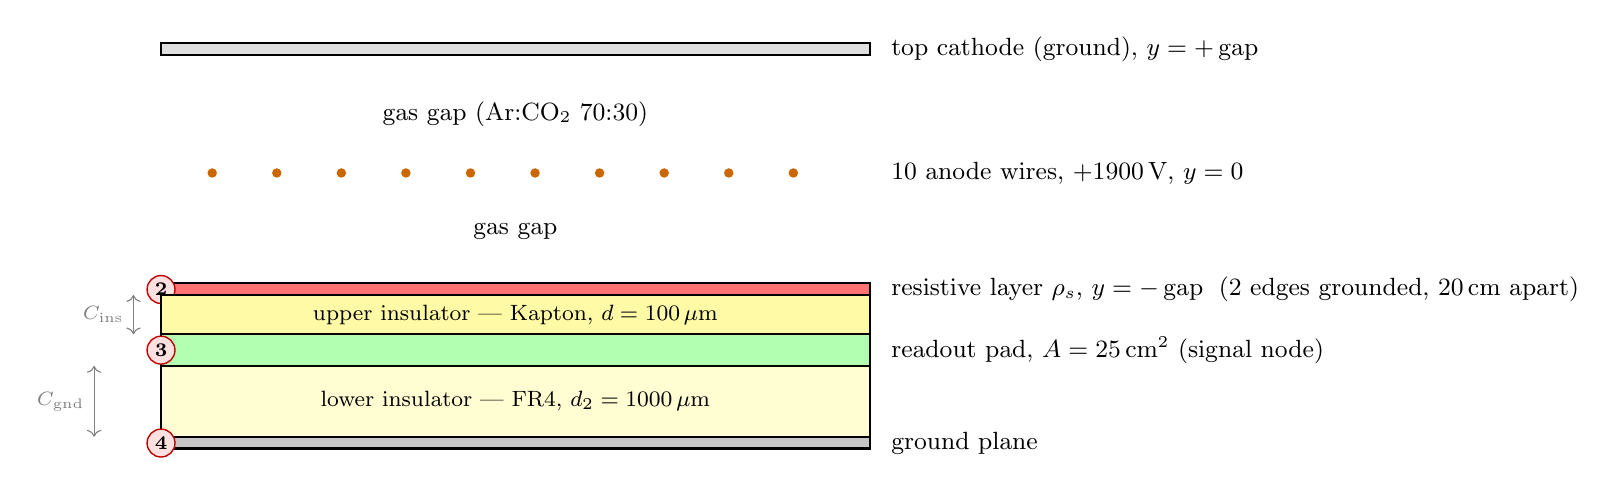
\begin{tikzpicture}[x=1cm,y=1cm]
  \def\W{9}      % stack width
  % --- top cathode (ground) ---
  \draw[layer,fill=gray!25] (0,6.0) rectangle (\W,6.15);
  \node[right] at (\W+0.15,6.07) {\small top cathode (ground), $y=+\,$gap};
  % gas gap (upper half)
  \node at (\W/2,5.25) {\small gas gap (Ar:CO$_2$ 70:30)};
  % --- anode wires ---
  \foreach \i in {0,...,9}{\fill[orange!80!black] (0.65+0.82*\i,4.5) circle (0.06);}
  \node[right] at (\W+0.15,4.5) {\small 10 anode wires, $+1900$\,V, $y=0$};
  % gas gap (lower half)
  \node at (\W/2,3.75) {\small gas gap};
  % --- resistive layer (gas boundary = stop surface) ---
  \draw[layer,fill=red!55] (0,2.95) rectangle (\W,3.10);
  \node[right] at (\W+0.15,3.02)
       {\small resistive layer $\rho_s$, $y=-\,$gap \;(2 edges grounded, 20\,cm apart)};
  \node[critmark] at (-0.0,3.02) {2};
  % --- upper insulator (Kapton 100 um) ---
  \draw[layer,fill=yellow!35] (0,2.45) rectangle (\W,2.95);
  \node at (\W/2,2.70) {\footnotesize upper insulator — Kapton, $d=100\,\mu$m};
  % --- readout pad ---
  \draw[layer,fill=green!30] (0,2.05) rectangle (\W,2.45);
  \node[right] at (\W+0.15,2.25) {\small readout pad, $A=25$\,cm$^2$ (signal node)};
  \node[critmark] at (-0.0,2.25) {3};
  % --- lower insulator (FR4 1 mm) ---
  \draw[layer,fill=yellow!18] (0,1.15) rectangle (\W,2.05);
  \node at (\W/2,1.60) {\footnotesize lower insulator — FR4, $d_2=1000\,\mu$m};
  % --- ground plane ---
  \draw[layer,fill=gray!45] (0,1.0) rectangle (\W,1.15);
  \node[right] at (\W+0.15,1.07) {\small ground plane};
  \node[critmark] at (-0.0,1.07) {4};
  % capacitor bracket annotations on the left
  \draw[<->,gray] (-0.35,2.95) -- (-0.35,2.45) node[midway,left,font=\scriptsize]{$C_{\rm ins}$};
  \draw[<->,gray] (-0.85,2.05) -- (-0.85,1.15) node[midway,left,font=\scriptsize]{$C_{\rm gnd}$};
\end{tikzpicture}
\end{center}

\noindent\textbf{Induced pad signal (Shockley–Ramo).} The pad weighting potential is the
\emph{infinite}-plane wire-screened cathode potential scaled by a lumped capacitive divider
\[
  W_{\rm pad}(x,y)=\alpha\,W_{\rm cathode}(x,y),\qquad
  \alpha=\frac{C_{\rm ins}}{C_{\rm ins}+C_{\rm gap}+C_{\rm gnd}},\quad
  C_{\rm ins}=\tfrac{\varepsilon_r}{d},\;C_{\rm gap}=\tfrac1{\rm gap},\;
  C_{\rm gnd}=\tfrac{\varepsilon_{r2}}{d_2}.
\]
For the default config $\alpha=0.868$ (0.980 with no ground plane). \crit{3}\,\crit{4} The finite
pad area and the ground plane enter \emph{only} through $\alpha$ and the input capacitance —
the weighting-field \emph{shape} is still the infinite plane.

\vspace{2mm}
\noindent\textbf{(B) Per-channel processing chain (block diagram, left $\to$ right)}
\begin{center}
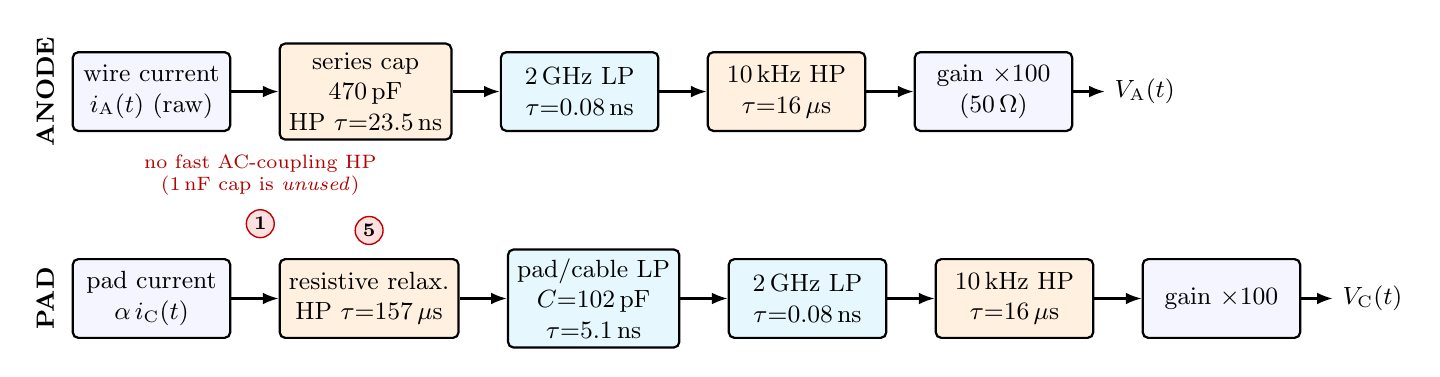
\begin{tikzpicture}[x=1cm,y=1cm,node distance=4mm and 6mm]
  % ===== ANODE (wire) channel =====
  \node[blk]                         (aIn)  {wire current\\$i_{\rm A}(t)$ (raw)};
  \node[hp,right=of aIn]             (aHP1) {series cap\\470\,pF\\HP $\tau{=}23.5$\,ns};
  \node[lp,right=of aHP1]            (aLP)  {2\,GHz LP\\$\tau{=}0.08$\,ns};
  \node[hp,right=of aLP]             (aHP2) {10\,kHz HP\\$\tau{=}16\,\mu$s};
  \node[blk,right=of aHP2]           (aG)   {gain $\times100$\\($50\,\Omega$)};
  \node[right=4mm of aG,font=\small] (aOut) {$V_{\rm A}(t)$};
  \draw[sig] (aIn)--(aHP1); \draw[sig](aHP1)--(aLP); \draw[sig](aLP)--(aHP2);
  \draw[sig] (aHP2)--(aG);  \draw[sig](aG)--(aOut);
  \node[left=1mm of aIn,font=\small\bfseries,rotate=90,anchor=south] {ANODE};

  % ===== CATHODE (pad) channel =====
  \node[blk,below=16mm of aIn]       (cIn)  {pad current\\$\alpha\,i_{\rm C}(t)$};
  \node[hp,right=of cIn]             (cRel) {resistive relax.\\HP $\tau{=}157\,\mu$s};
  \node[lp,right=of cRel]            (cILP) {pad/cable LP\\$C{=}102$\,pF\\$\tau{=}5.1$\,ns};
  \node[lp,right=of cILP]            (cLP)  {2\,GHz LP\\$\tau{=}0.08$\,ns};
  \node[hp,right=of cLP]             (cHP)  {10\,kHz HP\\$\tau{=}16\,\mu$s};
  \node[blk,right=of cHP]            (cG)   {gain $\times100$};
  \node[right=4mm of cG,font=\small] (cOut) {$V_{\rm C}(t)$};
  \draw[sig] (cIn)--(cRel); \draw[sig](cRel)--(cILP); \draw[sig](cILP)--(cLP);
  \draw[sig] (cLP)--(cHP);  \draw[sig](cHP)--(cG); \draw[sig](cG)--(cOut);
  \node[left=1mm of cIn,font=\small\bfseries,rotate=90,anchor=south] {PAD};

  % missing fast AC-coupling marker between cRel and cILP
  \node[critmark] at ($(cIn)!0.5!(cRel)+(0,0.95)$) (m1) {1};
  \node[red!70!black,font=\scriptsize,above=0.5mm of m1,align=center]
       {no fast AC-coupling HP\\(1\,nF cap is \emph{unused})};
  \node[critmark] at ($(cRel.north)+(0,0.35)$) {5};
\end{tikzpicture}
\end{center}

\noindent The anode chain is high-passed at $\tau=23.5$\,ns (the 470\,pF series cap), so its
output is a fast (differentiated) pulse. The pad chain's only high-passes are the resistive
relaxation ($\tau=157\,\mu$s) and the amplifier's intrinsic 10\,kHz edge ($\tau=16\,\mu$s) —
\emph{both far slower than the few-$\mu$s ion-drift tail}, so the pad output keeps the full
slow unipolar tail.

\vspace{2mm}
\noindent\textbf{(C) Component-level electronics — faithful current amplifier, then integrate its output}
\begin{center}
\resizebox{\textwidth}{!}{%
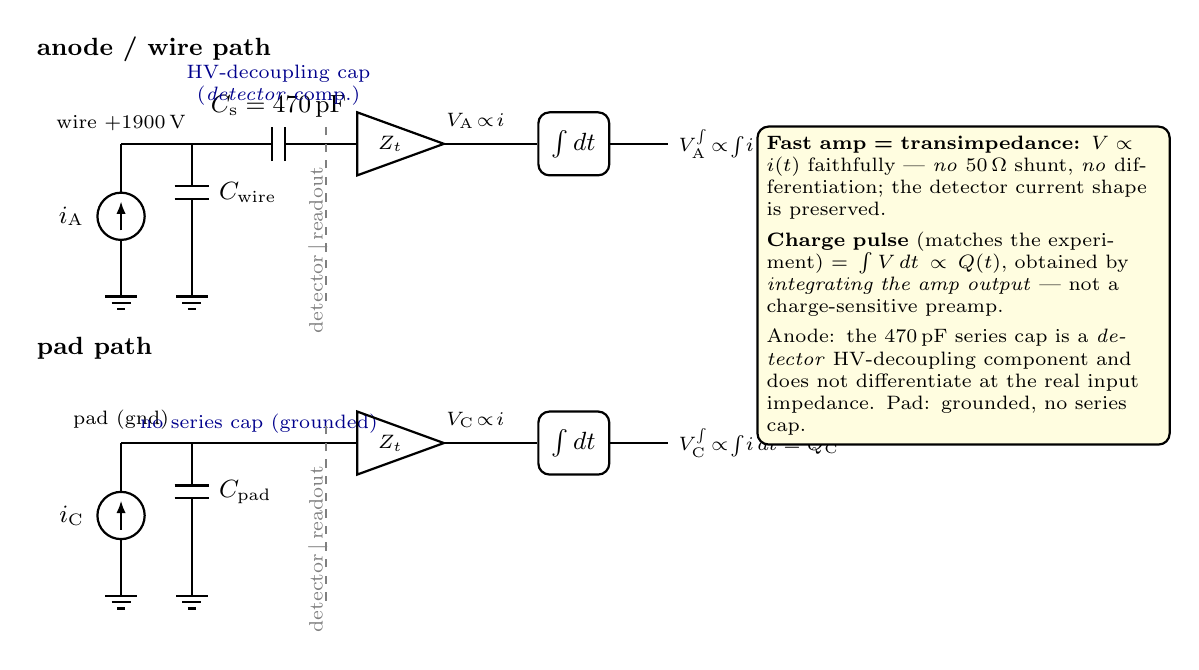
\begin{tikzpicture}[x=1cm,y=1cm,thick,font=\small]
  % ===== Row 1: ANODE / wire path =====
  \node[anchor=west,font=\small\bfseries] at (-1.2,2.0){\textsc{anode / wire} path};
  \pic at (0,-1.0){gnd}; \draw (0,-1.0)--(0,-0.42);
  \draw (0,-0.12) circle (0.30);
  \draw[-{Latex[length=1.6mm]}] (0,-0.30)--(0,0.07);
  \node[left=0pt] at (-0.34,-0.12){$i_{\rm A}$};
  \draw (0,0.18)--(0,0.8); \node[above,align=center] at (0,0.84){\scriptsize wire $+1900$\,V};
  \draw (0,0.8)--(0.9,0.8);
  \pic at (0.9,0.18){capv};
  \draw (0.9,0.8)--(0.9,0.63); \draw (0.9,-0.27)--(0.9,-1.0); \pic at (0.9,-1.0){gnd};
  \node[right=1pt] at (1.08,0.18){$C_{\rm wire}$};
  \draw (0.9,0.8)--(1.55,0.8);
  \pic at (2.0,0.8){caph}; \node[above] at (2.0,1.0){$C_{\rm s}=470$\,pF};
  \node[align=center,font=\scriptsize,blue!55!black] at (2.0,1.55){HV-decoupling cap\\(\emph{detector} comp.)};
  \draw (2.45,0.8)--(3.0,0.8);
  \draw[dashed,gray] (2.6,-1.2)--(2.6,1.1);
  \node[gray,font=\scriptsize,rotate=90] at (2.5,-0.55){detector\,$|$\,readout};
  % transimpedance amp (no input shunt!)
  \draw (3.0,1.2)--(3.0,0.4)--(4.1,0.8)--cycle; \node at (3.42,0.8){\scriptsize $Z_t$};
  \draw (4.1,0.8)--(4.85,0.8); \node[above,font=\scriptsize] at (4.5,0.86){$V_{\rm A}\!\propto\! i$};
  \node[draw,rounded corners,minimum height=8mm,minimum width=9mm] (i1) at (5.75,0.8){$\int dt$};
  \draw (4.85,0.8)--(i1.west); \draw (i1.east)--(6.95,0.8);
  \node[right,font=\scriptsize] at (6.95,0.8){$V_{\rm A}^{\int}\!\propto\!\int\! i\,dt={Q_{\rm A}}$};

  % ===== Row 2: PAD path =====
  \begin{scope}[yshift=-3.8cm]
    \node[anchor=west,font=\small\bfseries] at (-1.2,2.0){\textsc{pad} path};
    \pic at (0,-1.0){gnd}; \draw (0,-1.0)--(0,-0.42);
    \draw (0,-0.12) circle (0.30);
    \draw[-{Latex[length=1.6mm]}] (0,-0.30)--(0,0.07);
    \node[left=0pt] at (-0.34,-0.12){$i_{\rm C}$};
    \draw (0,0.18)--(0,0.8); \node[above,align=center] at (0,0.84){\scriptsize pad (gnd)};
    \draw (0,0.8)--(0.9,0.8);
    \pic at (0.9,0.18){capv};
    \draw (0.9,0.8)--(0.9,0.63); \draw (0.9,-0.27)--(0.9,-1.0); \pic at (0.9,-1.0){gnd};
    \node[right=1pt] at (1.08,0.18){$C_{\rm pad}$};
    \node[align=center,font=\scriptsize,blue!55!black] at (1.75,1.05){no series cap (grounded)};
    \draw (0.9,0.8)--(3.0,0.8);
    \draw[dashed,gray] (2.6,-1.2)--(2.6,1.1);
    \node[gray,font=\scriptsize,rotate=90] at (2.5,-0.55){detector\,$|$\,readout};
    \draw (3.0,1.2)--(3.0,0.4)--(4.1,0.8)--cycle; \node at (3.42,0.8){\scriptsize $Z_t$};
    \draw (4.1,0.8)--(4.85,0.8); \node[above,font=\scriptsize] at (4.5,0.86){$V_{\rm C}\!\propto\! i$};
    \node[draw,rounded corners,minimum height=8mm,minimum width=9mm] (i2) at (5.75,0.8){$\int dt$};
    \draw (4.85,0.8)--(i2.west); \draw (i2.east)--(6.95,0.8);
    \node[right,font=\scriptsize] at (6.95,0.8){$V_{\rm C}^{\int}\!\propto\!\int\! i\,dt={Q_{\rm C}}$};
  \end{scope}

  % explanatory box
  \node[draw,rounded corners,fill=yellow!12,align=left,font=\scriptsize,text width=5.0cm]
       at (10.7,-1.0)
       {\textbf{Fast amp = transimpedance:} $V\!\propto\! i(t)$ faithfully — \emph{no} 50\,$\Omega$
        shunt, \emph{no} differentiation; the detector current shape is preserved.\\[3pt]
        \textbf{Charge pulse} (matches the experiment) $=\int V\,dt\propto Q(t)$, obtained by
        \emph{integrating the amp output} — not a charge-sensitive preamp.\\[3pt]
        Anode: the 470\,pF series cap is a \emph{detector} HV-decoupling component and does not
        differentiate at the real input impedance. Pad: grounded, no series cap.};
\end{tikzpicture}}
\end{center}

\vspace{1mm}
\hrule
\vspace{2mm}
\noindent\fcolorbox{green!55!black}{green!7}{\parbox{\dimexpr\textwidth-2\fboxsep-2\fboxrule}{%
\textbf{Model fix (implemented).} The mismatch was that the readout \emph{differentiated} the
current — a spurious $50\,\Omega$-input high-pass — whereas the measured pulse is an
\emph{integral} of the current. Resolution, \emph{without} a charge-sensitive preamp: the fast
amp is now a faithful \emph{transimpedance} stage, $V_{\rm amp}\propto i(t)$ (no input-network
RC, no differentiation), and the measured charge pulse is reproduced by \textbf{integrating the
amp output}, $V^{\int}(t)=\int V_{\rm amp}\,dt\propto Q(t)$. The simulation writes both the
faithful current (\texttt{p\_anode\_amp} / \texttt{p\_cathode\_amp}) and its integral
(\texttt{p\_anode\_amp\_int} / \texttt{p\_cathode\_amp\_int}, the charge pulse to compare with
the measurement).}}

\vspace{2mm}
\noindent\textbf{Remaining criticalities}
\begin{enumerate}\setlength\itemsep{1pt}
\item[\crit{1}] \textbf{The anode series capacitor is a \emph{detector} component (now handled).}
  The 470\,pF in series with the wire (\texttt{wire\_series\_cap\_pf}) is the detector's
  HV-decoupling capacitor — the wire sits at $+1900$\,V and its signal is AC-coupled off the
  bias through it, present for \emph{any} readout. The earlier model wrongly applied it as a
  $50\,\Omega$ amplifier-input high-pass ($\tau{=}23.5$\,ns) that differentiated the wire
  signal; that high-pass (and the pad input-cap low-pass) have been \emph{removed} — the amp is
  now a faithful transimpedance, and at the real input impedance this cap does not differentiate
  on the signal timescale. \texttt{coupling\_cap\_nf} (1\,nF) remains \emph{legacy/unused}.
\item[\crit{2}] \textbf{Resistive layer = gas boundary only.} It is the analytic cathode plane
  at $y=-$gap; charge is correctly stopped there, but it is treated as a transparent
  dielectric interface for the prompt signal (the $\alpha$ divider), not a true resistive
  boundary solved in the field.
\item[\crit{3}] \textbf{Finite pad area is not in the weighting field.} $A=25$\,cm$^2$ only
  rescales amplitude (via $\alpha$ and input $C$); the weighting potential is still the
  infinite plane. A real finite pad localizes the weighting potential, which largely
  \emph{cancels} the fast electron spike and changes the pulse shape — not captured.
\item[\crit{4}] \textbf{Ground plane folded into $\alpha$.} The grounded backplane is modeled
  as a lumped $C_{\rm gnd}$ that scales the prompt amplitude ($\alpha:0.98\to0.87$) plus an
  input load; it does not change the weighting-field geometry (a layered field solve would).
\item[\crit{5}] \textbf{Relaxation $\tau=157\,\mu$s} $\gg$ the ion tail and $\gg$ the
  40\,$\mu$s window, so the "delayed signal" feature is effectively inactive at these
  parameters — it neither shapes nor differentiates the pad pulse.
\item[\crit{6}] \textbf{Modelling approximations.} The amplifier is now an ideal transimpedance
  with only the intrinsic 2\,GHz upper pole ($\tau=0.08$\,ns, inactive at the 0.1\,ns bin size)
  and gain — not the full CIVIDEC transfer function. The $N\approx227$ primaries are deposited
  at one point, making the electron spike artificially narrow ($\sim0.2$\,ns vs $\sim3$\,ns) —
  this affects the \emph{current} shape (and hence its integral), not the integrate question.
\end{enumerate}

\noindent\textbf{Status.} The front-end fix is implemented: a faithful transimpedance amp
($V_{\rm amp}\propto i$) plus an integrated output ($\int V_{\rm amp}\,dt\propto Q$) — no
charge-sensitive preamp, no $50\,\Omega$-input differentiation. Items \crit{2}–\crit{6}
(resistive-layer / dielectric lumping and the point-deposit approximation) remain and shape the
current that is integrated, not the integrate-vs-differentiate behaviour.
\end{document}
